\documentclass{article}
\usepackage[tmargin=1in,bmargin=1in,lmargin=1.5in,rmargin=1.5in]{geometry}
\usepackage{amsfonts,amsmath,amssymb,amsthm}
\usepackage{mathrsfs}
\usepackage{ccfonts}
\usepackage{relsize,fancyhdr,parskip}
\usepackage{graphicx}

\usepackage{tikz} \usetikzlibrary{shapes, shapes.geometric,
  shapes.symbols, shapes.arrows, shapes.multipart, shapes.callouts,
  shapes.misc,decorations.markings,decorations.shapes}

\pagestyle{fancy}
\lhead{Ben Carriel}
\chead{Math 6510 Problem Set 4}
\rhead{\today}

\parskip 7.2pt
\parindent 8pt

\newcommand{\tab}{\hspace*{2em}}
\newcommand{\tand}{\tab\text{and}\tab}

\DeclareMathOperator{\N}{\mathbb{N}}
\DeclareMathOperator{\Z}{\mathbb{Z}}
\DeclareMathOperator{\Q}{\mathbb{Q}}
\DeclareMathOperator{\R}{\mathbb{R}}
\DeclareMathOperator{\C}{\mathbb{C}}
\DeclareMathOperator{\D}{\mathbb{D}}
\DeclareMathOperator{\T}{\mathbb{T}}
\DeclareMathOperator{\capchi}{\raisebox{2pt}{$\mathlarger{\mathlarger{\chi}}$}}

%\DeclareMathOperator{\divides}{\mathrel{|}}
\DeclareMathOperator{\suchthat}{\mathrel{:}}

\DeclareMathOperator{\lra}{\longrightarrow}
\DeclareMathOperator{\into}{\hookrightarrow}
\DeclareMathOperator{\onto}{\twoheadrightarrow}
\DeclareMathOperator{\bijection}{\leftrightarrow}
\DeclareMathOperator{\lap}{\bigtriangleup}

\newcommand{\problem}[1]{\noindent{\textbf{Problem #1}}\\}
\newcommand{\problempart}[1]{\noindent{\textbf{(#1)}}}
\newcommand{\exercise}[1]{\noindent{\textbf{Exercise #1:}}}

\newcommand{\der}[2]{\frac{\partial #1}{\partial #2}}
\newcommand{\norm}[1]{\|#1\|}
\newcommand{\diam}[1]{\text{diam}(#1)}
\newcommand{\seq}[2]{\{#1_{#2}\}_{#2 = 1}^\infty}

\newcommand{\conj}[1]{\overline{#1}}
\newcommand{\cis}[1]{\operatorname{cis}#1}
\newcommand{\res}{\operatorname{res}}


\newcommand{\real}{\mathrel{\text{Re}}}
\newcommand{\imag}{\mathrel{\text{Im}}}
\newtheorem*{thm}{\\ Theorem}
\newtheorem*{lem}{\\ Lemma}
\newtheorem*{claim}{\\ Claim}
\newtheorem*{defn}{\\ Definition}
\newtheorem*{prop}{\\ Proposition}

\begin{document}
\exercise{1.3.5}

We will use the tube lemma to produce such a neighborhood of the left
edge. Let $p: \tilde{X} \to X$ be a covering space. We must find
points that are ``close-enough'' in the lift to the inverse image of
the left most line. More precisely, if we consider the function $pd:
\tilde{X}\times \tilde{X} \to X$ given by $(x,y) \mapsto
d(p(x),p(y))$, then because $p$ is locally injective (locally a
homeomorphism for a good enough cover by the definition), we can find
an open neighborhood of the point $(x,x) \in \tilde{X}\times
\tilde{X}$ for $x$ in the inverse image of the left line $U_x \times
U_x$ such that
\[
(U_x \times U_x) \cap pd^{-1}(0)^c \subset \{(y,y) \suchthat y\in \tilde{X}\}
\]
Then we use the compactness of the left line $\ell \subset X$ to see
that its inverse image $\ell^{-1}$, must also be compact and the set
\[
U = \bigcup_{y = pd^-1{x}} (U_d \times U_d)
\]
is an open cover. So we see that $\ell^{-1}\times \ell^{-1}$ is
contained in $U \cup pd^-1(0)$ by the above. Now we can apply the tube
lemma to find open $V_1,V_2$ such that
\[
\ell^{-1}\times \ell^{-1} \subset V_1 \times V_2 \subset U \cup pd^-1(0)
\]
Then clearly $V = V_1 \cap V_2$ is a desired enighborhood by
construction.

% FIX THIS
To see that $X$ has no simply connected covering space, we observe
that any open neighborhood of the left line necessarily intersects
finitely many of the lines $\{1/n\} \times I$. And so is homeomorphic
to a disjoint union of intervals. Consequently, $X$ is not locally
path-connected. Then the classification theorem for covering spaces is
violated and so $X$ cannot have a simply connected covering space.

\exercise{1.3.6}

We are initially given the following covering space $\tilde{X}$ of the
shrinking wedge of circles:
\begin{figure}[h!]
  \centering
  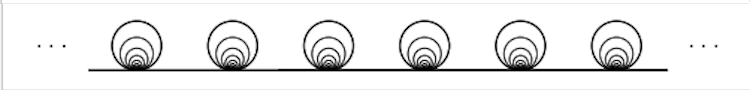
\includegraphics[scale=0.5]{onesheet.png}
  \caption{The initial covering space, $\tilde{X}$}
\end{figure}

We create the covering map as follows: the bottom line is identified
with $\R$ and becomes the usual covering space of the outer circle in
an individual covering of the shrinking wedge. Each of the circles, of
radius $1/n$ is identified with the circle of radius $1/(n+1)$ in the
base space. This is clearly a covering space map as the inverse of
every open set is a disjoint union of copies in the covering space.

Now we will create a 2-sheeted cover, $Y$ of the space $\tilde{Y}$. By
gluing two identical copies together in the following way:
\begin{figure}[h!]
  \centering
  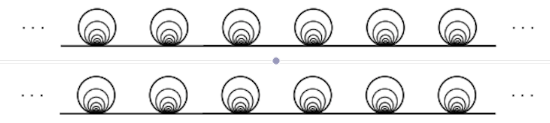
\includegraphics[scale=0.5]{twosheet.png}
  \caption{The covering space of $\tilde{X}$, $Y$}
\end{figure}
We then define the map in the following way:
\begin{enumerate}
\item Send one of the base lines (say the bottom one) in $Y$ to the
  base line in $\tilde{X}$.
\item Send the edge $(v_n,v_{n+1})$ in the other base line to the
  outermost loop of the $n^{\text{th}}$ wedge in $\tilde{X}$, where
  $v_n$ is the common vertex to all of the shrinking wedges in the
  copy of $X$.
\item Send each pair of shrinking wedges in $Y$ to the corresponding
  wedge in $\tilde{X}$ (map the aligned copies to the top one in the
  diagram) in such a way that the loop of radius $1/n$ is sent to a
  loop of radius $1/(n+1)$
\end{enumerate}
To see that this is a covering map we note that any open set in $X$
lifts to two open sets in $Y$. If the open set is on the base line, it
lifts to a copy of itself in one base line of $Y$ as well as an outer
circle of one of the wedges in $Y$. Otherwise, it is in a wedge and is
sent to the corresponding copies of itself in $Y$ but one loop inward
as described above. This is a two sheeted cover.

To see that the composition of maps $q: Y \to \tilde{X}$ and
$p:\tilde{X}\to X$ is not a covering space consider the common vertex
of loops in $X$, call it $x$. Then we can lift any neighborhood $U$ of
$x$ via $p^{-1}$ to a set of neighborhoods in $\tilde{X}$ about the
set of basepoints of each copy of $X$. We then lift each of these
neighborhoods into $Y$. Because the points to adjacent to
$(p^{-1}(x))_n$ will map to different wedges, depending on which side
they were on (rule 2 described above),

\exercise{1.3.7}



\exercise{1.3.9}

Let $X$ be a path connected, locally path-connected space such that
$\pi_1(X)$ is finite. If we look at the induced homomorphism $f_*:
\pi_1(X) \to \pi_1(S^1)$ we see that $f_*(\pi_1(X))$ is a finite
subgroup of $\pi_1(S^2) \cong \Z$, which means it is the trivial
group and $f_*$ is the trivial homomorphism.

Because $X$ is path-connected and locally path connected any map $f: X
\to S^1$ lifts to map $\tilde{f}:\R \to S^1$ such that $f =
p\tilde{f}$. Moreover, $\R$ is contractible, so the identity map in
$\R$ is homotopic to a constant map. But, $f_*(\pi_1(X)) \leq
p_*(\pi_1(\R))$ and $f_*$ is the identity, so it must be homotopic to a
constant map and so any map in $X$ is homotopic to a constant.

\exercise{1.3.11}

Consider a graph that is one vertex, with a 4-cycle $a,b,c,d$ incident
to that vertex. Connect each of the vertices of these graphs by an
edge $e$ (note 1 vertex per graph, this is what will map to the
basepoint). Now what we will do is glue copies of these graphs
together, and only count one of every two of the base vertices as a
vertex in a new space $X$. This will be our covering space (so instead
of each diamond having a vertex, every other one does).

We can make two spaces for which this is a covering space: The first
is a graph that is one copy of the diamond along with a self edge $e$
at the vertex and a an edge along the diagonal (making the triangle
$a,b,e$). The second graph will be a a collection of diamonds with two
diagonal edges making the $a,b,e$ and $e,c,d$ triangles. Moreover, we
will add a vertex at $a,b$ so that this is now a relation. Note that in
this second case, the covering map is not surjective (it points out
that the cover need not be surjective in the text).

It is clear that both of the above spaces have $X$ as a covering space
because all of the relations are preserved in the covering map and
each set of intervals will map to a discrete set in $X$, however no
space can have both of the above as a covering space because that
would require adding the relations that are contradictory to one
another.

\exercise{1.3.23}

Because the action is properly discontinuous for each $x$ we can find
an open set $U$ containing $x$ such that $g(U) \cap U$ is non-empty
for only finitely many $g$. Suppose that $g_1,g_2,\ldots,g_n$ are the
elements such that $g(U)\cap U = \emptyset$. Now we use the Hausdorff
property to find an open set $V_0 \subset U$ such that $g_i(U) \cap
V_0 = \emptyset$ for each $i$. We iterate this process for each of the
$g_i$ (the Hausdorff property guarantees we can do this finitely many
times by induction) to find sets $V_j \subset g_j(U)$ containing $x$
that are all disjoint. Then we set
\[
W = \bigcap_{j=0}^{n} g_j^{-1}(V_j \cap g_j(V_0))
\]
Then $W$ contains $X$ and the $g(W)$ are pariwise disjoint for all $g
\in G$.

\exercise{A1}
\begin{enumerate}
\item[\textbf{(a)}]
\item[\textbf{(b)}]
\end{enumerate}

\exercise{A2}
\begin{enumerate}
\item[\textbf{(a)}]
\item[\textbf{(b)}]
\end{enumerate}
\end{document}